% Requirements 1/  :Summary
\begin{frame}
	\centering
	\frametitle{Introducing Repo-Rover!}
	\begin{block}{Summary}
		Repo-Rover will traverse a user's filesystem from given a root address, locate all Git repos contained therein, and provide relevant diagnostic information to the user.
	\end{block}
	
	\resizebox{11cm}{2.5cm}{%
	\begin{tikzpicture} [node distance = 7em]
		\node[entity] (system) {Filesystem};
		\node[relationship] (contains) [right of=system, node distance = 10 em] {Contains} edge node[auto, swap] {1} (system);		
		
		% Middle branch
		\node[entity] (repo) [right of=contains, node distance = 10 em] {Git Repo} edge[total] node[auto, swap] {n} (contains);

		\node[attribute] (mid_feature1) [above right of=repo, node distance = 5 em] {\discriminator{Feature 1}} edge (repo);
		\node[attribute] (mid_feature2) [right of=repo, node distance = 7 em] {\discriminator{Feature 2}} edge (repo);
		\node[attribute] (mid_feature3) [below right of=repo, node distance = 5 em] {\discriminator{Feature 3}} edge (repo);
	\end{tikzpicture}
	}
	
		\pause
	\begin{block}{Purpose}
			To provide an easy, automated means for computer scientists to monitor their Git repositories and avoid potentially costly oversights.
	\end{block}
\end{frame}

% Requirements 2/  :Constraints
\begin{frame}
	\centering
	\frametitle{Requirements}
	\resizebox{11cm}{3.0cm}{%
			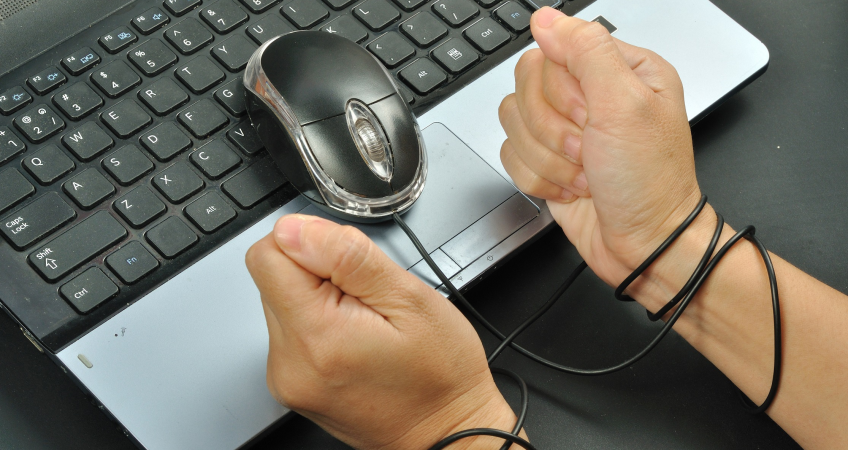
\includegraphics[]{images/constraints.png}	
	} %end resizebox
	
	\begin{block}{Process Constraints}
		\begin{enumerate}
			\item Incremental Development
			\item Documentation
			\item Public Access
		\end{enumerate}
	\end{block}
	\pause
	\begin{block}{Design Constraints}
		\begin{enumerate}
			\item Audience
			\item Operating System
			\item Programming Language
		\end{enumerate}
	\end{block}
\end{frame}

% Requirements 3 /
\begin{frame}
	\centering
	\frametitle{Requirements}
	\resizebox{11cm}{3.0cm}{%
		
\includegraphics[]{images/functional.png}
	}
	
	\begin{block}{Functional Requirements}
		\begin{enumerate}
			\item <1-> Filesystem Traversal
			\item <2->Diagnostic Summary (\textbf{Per} Repo)
			\pause
			\begin{itemize}
				\item <2-> Files with untracked modifications
				\item <2-> Files in staging area
				\item <2-> Committed files not pushed
			\end{itemize}
			\item <3-> Diagnostic Summary (\textbf{All} Repos)
			\begin{itemize}
				\item <3-> Total number of repos
				\item <3-> Percentage of "clean" repos
			\end{itemize}
		\end{enumerate}		
	\end{block}
	

\end{frame}

\begin{frame}
	\centering
	\frametitle{Requirements}
	
    \resizebox{11cm}{3.0cm}{
	    \includegraphics{images/quality.jpg}
	} % end resizebox 
	
	\begin{block}{Non-Functional Requirements}
		\begin{enumerate}
			\item <1->Scalability
			\item <2-> Speed
			\item <3-> Ease of Use
			\item <4-> Reliability
		\end{enumerate}		
	\end{block}
	
	\vspace{1.5cm}
\end{frame}